\documentclass{ximera}
\graphicspath{     %% setup a global graphics path
{./}               %% look in the same-level directory
{./pictures/}      %% look in graphics
{../pictures/}     %% look up one directory, then in graphics
%{../../pictures/} %% look up two directories, then in graphics
}

\author{Zack Reed}
%borrowed from ximera interactive la
\title{Determinants and Geometry}
\begin{document}
\begin{abstract}

\end{abstract}
\maketitle


\section*{Determinants, Areas, and Volumes}

So far, we've focused much of this chapter on determining properties of matrices and specifically whether or not they are invertible. 

We now introduce a very related topic that also has farther reaching implications for matrices as well, beyond invertibility, and is an important measure for Chapters 7, 8, and 9.

An intuition we've been discussing for whether matrices are invertibile is that when linear transformations ``squish'' space down to a smaller dimension, they are not invertible. One way to determine whether this ``squishing'' occurs is to measure by how much units of volume are stretched or compressed through the transformation. 

Consider, for instance, the matrix $\begin{bmatrix}
  3&0&0\\0&2&0\\0&0&1
\end{bmatrix}$. This stretches the $x$-axis by a factor of $3$ and the $y$-axis by a factor of $2$, as you can see in the following GeoGebra applet. Check the ``Adjust Matrix'' box and enter the columns of the matrix accordingly (note that the column vectors are listed as rows when being entered, so really you're entering the transpose of the matrix).

\begin{center}
  \geogebra{mdes5d4h}{858}{509}
\end{center}

As you can see, $A$ stretches out vectors in both the $x$ and $y$ directions while preserving the height. More importantly, the original $1\times1\times1$ cube becomes a stretched out rectangle, and the ``Transformed Volume'' measure reads as $6$. This means that the transformation stretches out space by a factor of $6$. 

If instead you enter the mug-squishing matrix $A=\begin{bmatrix}
  1&0&1\\0&2&2\\1&2&3
\end{bmatrix}$, you see the original cube squished down into a plane. 

The transformed volume of the unit cube is thus $\answer{0}$.

This gives us a clear way to determine whether linear transformations are invertible! Measuring this transformed volume is called finding \emph{the determinant}. The determinant arises from systematically extending the notions of areas and volumes to give clear ways of measuring volume-stretching and volume-compressing for any matrix transformation.

We will start with a $2$-dimensional approach to finding the area shifted by a transformation, and then build up to a $3$-dimensional volume shift. Higher-dimensional hypervolume shifts are just generlizations of what is done in $2$ and $3$ dimensions, and beyond $2$-dimensions the computations become rather cumbersome, so we will largely use MATLAB to compute determinants in practice. 


    \subsection*{$2\times 2$ Determinant and the Area of a Parallelogram}
     
    Consider the parallelogram determined by vectors $\vec{u}$ and $\vec{v}$.
     
    \begin{center}
    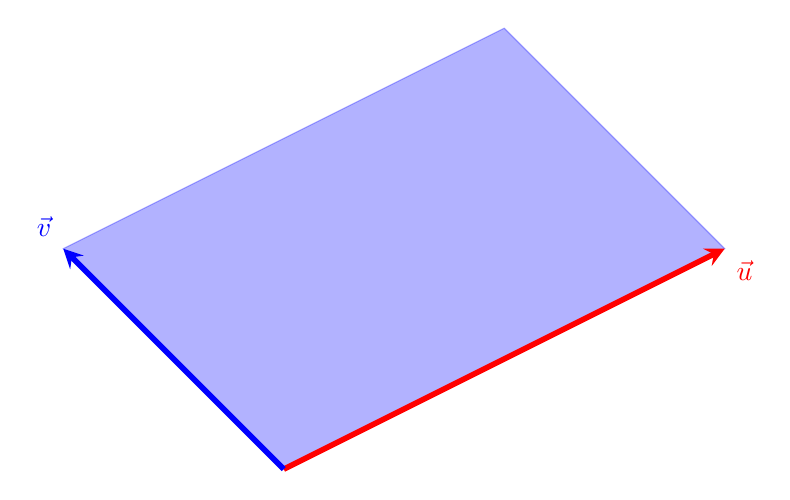
\begin{tikzpicture}[scale=1.4]
     
      \filldraw[blue, opacity=0.3](0,0)--(-2,2)--(2,4)--(4,2)--cycle;
     
    \draw[line width=2pt,red,-stealth](0,0)--(4,2) node[below right]{$\vec{u}$};
      
      \draw[line width=2pt,blue, -stealth](0,0)--(-2,2) node[above left]{$\vec{v}$};
    \end{tikzpicture}
    \end{center}

    $\vec{u}$ and $\vec{v}$ do not form a simple rectangle, and their orientation makes it initially cumbersome to get a parallelogram height and width for an area determination. 

    We can, however, cleverly set up a rectangular area from which we can use the coordinates of the vectors to determine the parallelogram area. This at first will be a bit laborious, but this process will work for any vector-spanning parallelogram and will also give us a means of defining the determinant!

    \begin{example}\label{ex:areaofparallelogram}
      First, let's draw the parallelogram within a grid.

      \begin{center}
      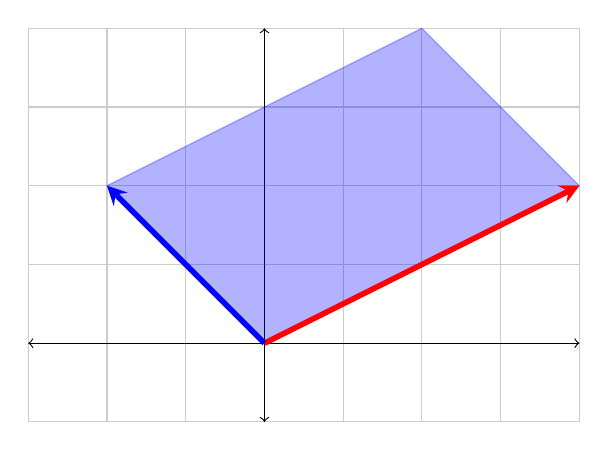
\begin{tikzpicture}[scale=1]
      \draw[thin,gray!40] (-3,-1) grid (4,4);
        \draw[<->] (-3,0)--(4,0);
        \draw[<->] (0,-1)--(0,4);
          
        \filldraw[blue, opacity=0.3](0,0)--(-2,2)--(2,4)--(4,2)--cycle;
        
      \draw[line width=2pt,red,-stealth](0,0)--(4,2);
        
        
       \draw[line width=2pt,blue,-stealth](0,0)--(-2,2);
         
      \end{tikzpicture}
      \end{center}

      \begin{explanation}

      The vectors that determine the parallelogram are
      $$\begin{bmatrix}4\\2\end{bmatrix}\quad\text{and}\quad\begin{bmatrix}-2\\2\end{bmatrix}$$

      The goal is to figure out the area of the parallelogram using just information from the two vectors. 

      As said earlier, we're going to put the parallelogram within a larger rectangle (using the vector coordinates), which will conveniently give us other geometric quantities from which we extract the paralellogram area!

      Let's create a rectangle that fully encompasses the parallelogram. The base of the rectangle will be the sum of the $x$-coordiantes, and the height will be the sum of the $y$-coordinates. This is true for any pair of vectors, and the key is that the vector $\vec{u}+\vec{v}$ determines the coordinates of the far tip. 

      Because this will generalize to any pair of vectors, let's use $\vec{u}=\begin{bmatrix}
        a\\c
      \end{bmatrix}$ and $\vec{v}=\begin{bmatrix}
        b\\d
      \end{bmatrix}$ as general stand-ins, and then at the end fill in our specific numbers.

      \begin{center}
        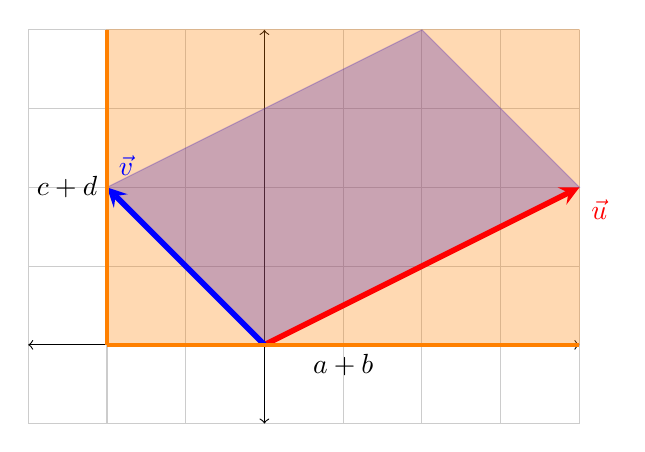
\begin{tikzpicture}[scale=1]
        \draw[thin,gray!40] (-3,-1) grid (4,4);
          \draw[<->] (-3,0)--(4,0);
          \draw[<->] (0,-1)--(0,4);
            
          \filldraw[blue, opacity=0.3](0,0)--(-2,2)--(2,4)--(4,2)--cycle;

              % Add the orange rectangle inscribing the parallelogram
          \filldraw[orange, opacity=.3] (-2,0) rectangle (4,4);
          
        \draw[line width=2pt,red,-stealth](0,0)--(4,2)node[below right]{$\vec{u}$};
          
         \draw[line width=2pt,blue,-stealth](0,0)--(-2,2)node[above right]{$\vec{v}$};

             % Add thick orange lines for base and height
        \draw[orange, ultra thick] (-2,0) -- (4,0); % Base of the rectangle
        \draw[orange, ultra thick] (-2,0) -- (-2,4); % Height of the rectangle


        % Add labels
        \node[anchor=north] at (1,0) {\(a+b\)}; % Label for the x-axis
        \node[anchor=east] at (-2,2) {\(c+d\)}; % Label for the y-axis
           
        \end{tikzpicture}
        \end{center}

        Now, surrounding our parallelogram are four triangles, which actually break down quite nicely in terms of $a, b, c$, and $d$.

        The top left and bottom right triangles move along the vector $\vec{u}$, and so their dimensions come from the base $a$ and height $c$.

        START HERE
      
      \end{explanation}
      \end{example}
        

        
      \begin{formula}\label{form:areaofparallelogramdeterminant} Let $\vec{u}=\begin{bmatrix}a\\b\end{bmatrix}$ and $\vec{v}=\begin{bmatrix}c\\d\end{bmatrix}$ be vectors of $\RR^2$.  The area of the parallelogram determined by $\vec{u}$ and $\vec{v}$ is given by
      $$\mbox{Area}=\Big|{\det\begin{bmatrix}a&b\\c&d\end{bmatrix}}\Big|=\Big|\det\begin{bmatrix}a&c\\b&d\end{bmatrix}\Big|$$
      \end{formula}
        
      \begin{example}\label{exp:polyArea}
          Use Formula \ref{form:areaofparallelogramdeterminant} to find the area of the polygon shown below.
        \begin{center}
      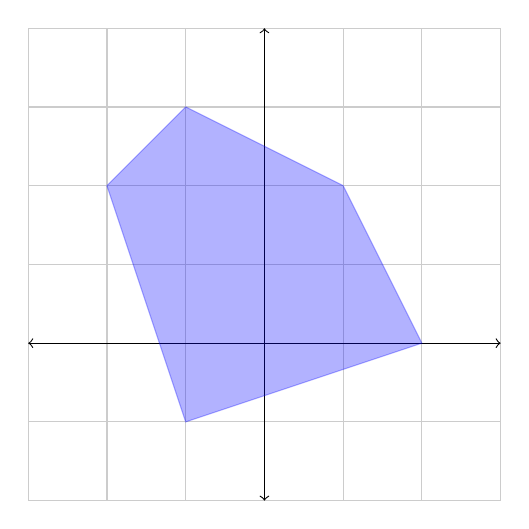
\begin{tikzpicture}[scale=1]
      \draw[thin,gray!40] (-3,-2) grid (3,4);
        \draw[<->] (-3,0)--(3,0);
        \draw[<->] (0,-2)--(0,4);
        \filldraw[blue, opacity=0.3](-1,-1)--(-2,2)--(-1,3)--(1,2)--(2,0)--cycle;
      %\draw[line width=2pt,red,-stealth](0,0)--(4,2);
      % \draw[line width=2pt,blue,-stealth](0,0)--(-2,2);
       \end{tikzpicture}
      \end{center}
      \begin{explanation}
          We will start by splitting this region into triangles.
          \begin{center}
      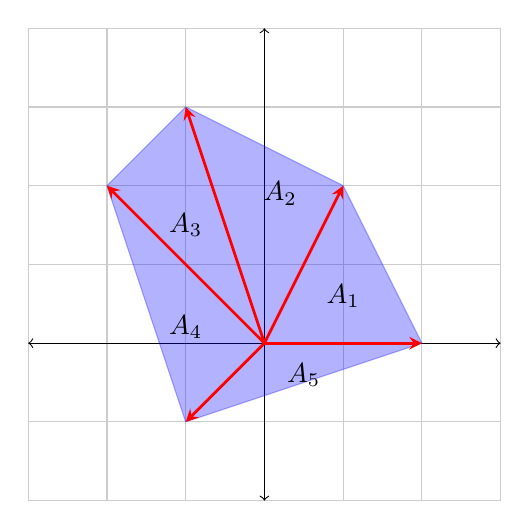
\begin{tikzpicture}[scale=1]
      \draw[thin,gray!40] (-3,-2) grid (3,4);
        \draw[<->] (-3,0)--(3,0);
        \draw[<->] (0,-2)--(0,4);
        \filldraw[blue, opacity=0.3](-1,-1)--(-2,2)--(-1,3)--(1,2)--(2,0)--cycle;
      \draw[line width=1pt,red,-stealth](0,0)--(-1,-1);
      \draw[line width=1pt,red,-stealth](0,0)--(-2,2);
      \draw[line width=1pt,red,-stealth](0,0)--(-1,3);
      \draw[line width=1pt,red,-stealth](0,0)--(1,2);
      \draw[line width=1pt,red,-stealth](0,0)--(2,0);
      \node[] at (1, 0.6)   (b) {$A_1$};
      \node[] at (0.2, 1.9)   (b) {$A_2$};
      \node[] at (-1, 1.5)   (b) {$A_3$};
      \node[] at (-1, 0.2)   (b) {$A_4$};
      \node[] at (0.5, -0.4)   (b) {$A_5$};
       \end{tikzpicture}
      \end{center}
          We can find the total area of the polygon by finding the area of each triangle.  The area of each triangle is half of the area of the corresponding parallelogram.  For instance, $A_1$ is half of the area of the parallelogram depicted below.
      \begin{center}
      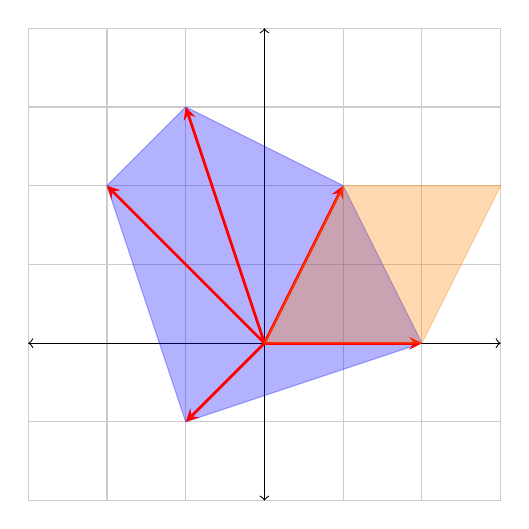
\begin{tikzpicture}[scale=1]
      \draw[thin,gray!40] (-3,-2) grid (3,4);
        \draw[<->] (-3,0)--(3,0);
        \draw[<->] (0,-2)--(0,4);
        \filldraw[blue, opacity=0.3](-1,-1)--(-2,2)--(-1,3)--(1,2)--(2,0)--cycle;
      \draw[line width=1pt,red,-stealth](0,0)--(-1,-1);
      \draw[line width=1pt,red,-stealth](0,0)--(-2,2);
      \draw[line width=1pt,red,-stealth](0,0)--(-1,3);
      \draw[line width=1pt,red,-stealth](0,0)--(1,2);
      \draw[line width=1pt,red,-stealth](0,0)--(2,0);
      \filldraw[orange, opacity=0.3](2,0)--(0,0)--(1,2)--(3,2)--cycle;
       \end{tikzpicture}
      \end{center}
      We compute
      $$A_1=\frac{1}{2}\left|\det\begin{bmatrix}2 & 1\\0 & 2\end{bmatrix}\right |=\answer{2}$$
      $$A_2=\frac{1}{2}\left|\det\begin{bmatrix}1 & -1\\2 & 3\end{bmatrix}\right |=\answer{2.5}$$
      $$A_3=\frac{1}{2}\left|\det\begin{bmatrix}-1 & -2\\3 & 2\end{bmatrix}\right |=\answer{2}$$
      $$A_4=\frac{1}{2}\left|\det\begin{bmatrix}-2 & -1\\2 & -1\end{bmatrix}\right |=\answer{2}$$
      $$A_5=\frac{1}{2}\left|\det\begin{bmatrix}-1 & 2\\-1 & 0\end{bmatrix}\right |=\answer{1}$$
      The total area of the polygon is $\answer{9.5}$.
      \end{explanation}
      \end{example}

  \end{document}
     
    \subsection*{$3\times 3$ Determinant and the Volume of a Parallelepiped}
     
    Our next goal is to find the volume of a three-dimensional figure called a \dfn{parallelepiped}.  A parallelepiped is a six-faced figure whose opposite faces are congruent parallelograms located in parallel planes.  A parallelepiped is a three-dimensional counterpart of a parallelogram, and is determined by three non-coplanar vectors in $\RR^3$.  The figure below shows a parallelepiped determined by three vectors.
     
    \begin{center}
    \tdplotsetmaincoords{70}{130}
    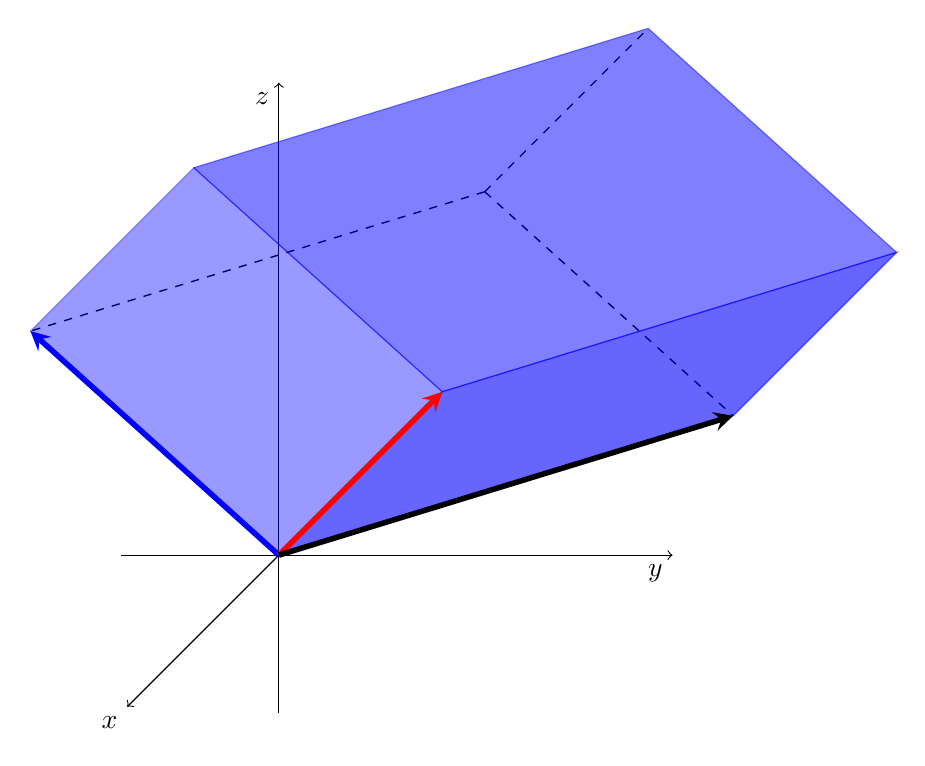
\begin{tikzpicture}
        \draw[->](-2,0,0)--(5,0,0) node[below left]{$y$};
        \draw[->](0,-2,0)--(0,6,0) node[below left]{$z$};
        \draw[->](0,0,-2)--(0,0,5) node[below left]{$x$};
         
        \draw[line width=0.5pt, dashed](3,5,1)--(5,1,-2);
        \draw[line width=0.5pt, dashed](3,5,1)--(-2,4,3);
        \draw[line width=0.5pt, dashed](3,5,1)--(7,9,6);
         
        \filldraw[blue, opacity=0.4] (0,0,0)--(-2, 4, 3)--(2,8,8)--(4,4,5)--cycle;
        \filldraw[blue, opacity=0.5] (2,8,8)--(4,4,5)--(9,5,3)--(7,9,6)--cycle;
        \filldraw[blue, opacity=0.6] (0,0,0)--(4,4,5)--(9,5,3)--(5,1,-2)--cycle;
         
        \draw[->, line width=2pt,blue, -stealth](0,0,0)--(-2,4,3);
        \draw[->, line width=2pt,red, -stealth](0,0,0)--(4,4,5);
        \draw[->, line width=2pt, -stealth](0,0,0)--(5,1,-2);
         
    \end{tikzpicture}
    \end{center}
     
    Consider a parallelepiped determined by vectors $\vec{u}$, $\vec{v}$ and $\vec{w}$, as shown below. 
     
    \begin{center}
    \tdplotsetmaincoords{70}{130}
    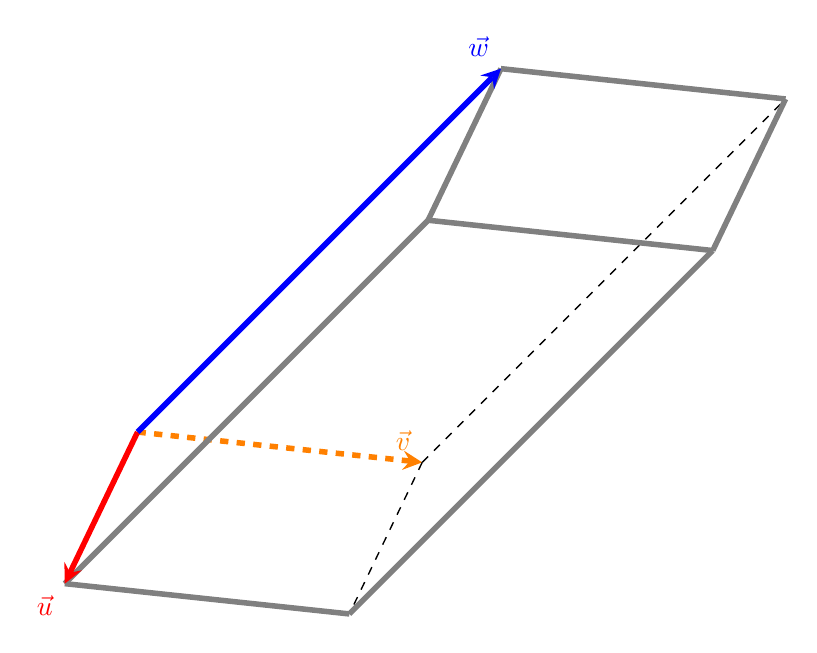
\begin{tikzpicture}
        \draw[->, line width=2pt, -stealth,orange,dashed](0,0,0)--(4,0,1)node[above left]{$\vec{v}$};
         
        \draw[line width=0.5pt, dashed](4,0,1)--(5,0,6);
        \draw[line width=0.5pt, dashed](4,0,1)--(9,5,2);
         
        \draw[line width=2pt, gray](1,0,5)--(6,5,6);
        \draw[line width=2pt, gray](10,5,7)--(6,5,6);
        \draw[line width=2pt, gray](10,5,7)--(5,0,6);
        \draw[line width=2pt, gray](1,0,5)--(5,0,6);
        \draw[line width=2pt, gray](6,5,6)--(5,5,1);
        \draw[line width=2pt, gray](9,5,2)--(5,5,1);
        \draw[line width=2pt, gray](10,5,7)--(9,5,2);
         
        \draw[->, line width=2pt,red, -stealth](0,0,0)--(1,0,5)node[below left]{$\vec{u}$};
        \draw[->, line width=2pt, blue, -stealth](0,0,0)--(5,5,1)node[above left]{$\vec{w}$} ;
       
    \end{tikzpicture}
    \end{center}
     
    The volume of a parallelepiped is given by
    $$\mbox{Volume}=(\text{area of base})(\text{height})$$
    We will consider the parallelogram determined by $\vec{u}$ and $\vec{v}$ to be the base of the parallelepiped.  Thus, the area of the base is given by
    $$\mbox{Area of Base}=\norm{\vec{u}\times\vec{v}}$$
    \begin{center}
    \tdplotsetmaincoords{70}{130}
    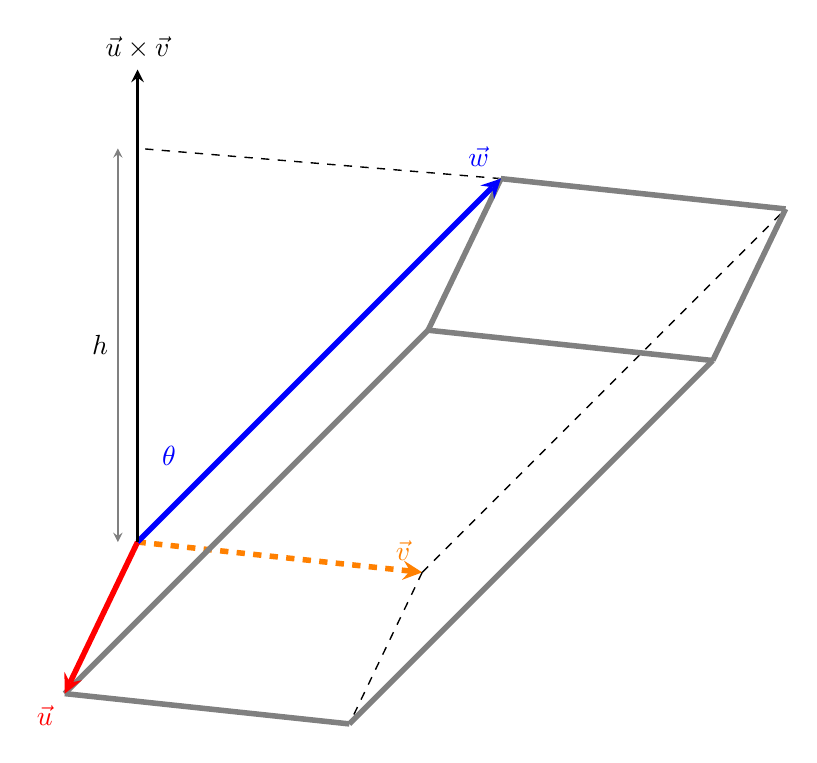
\begin{tikzpicture}
        \draw[->, line width=2pt, -stealth,orange,dashed](0,0,0)--(4,0,1)node[above left]{$\vec{v}$};
         
        \draw[line width=0.5pt, dashed](4,0,1)--(5,0,6);
        \draw[line width=0.5pt, dashed](4,0,1)--(9,5,2);
         
        \draw[line width=0.5pt, dashed](5,5,1)--(0,5,0);
         
        \draw[line width=2pt, gray](1,0,5)--(6,5,6);
        \draw[line width=2pt, gray](10,5,7)--(6,5,6);
        \draw[line width=2pt, gray](10,5,7)--(5,0,6);
        \draw[line width=2pt, gray](1,0,5)--(5,0,6);
        \draw[line width=2pt, gray](6,5,6)--(5,5,1);
        \draw[line width=2pt, gray](9,5,2)--(5,5,1);
        \draw[line width=2pt, gray](10,5,7)--(9,5,2);
         
        \draw[->, line width=2pt,red, -stealth](0,0,0)--(1,0,5)node[below left]{$\vec{u}$};
        \draw[->, line width=2pt, blue, -stealth](0,0,0)--(5,5,1)node[above left]{$\vec{w}$} ;
        \node[blue] at (0.4, 1.1)   (b) {$\theta$};
        \draw[->, line width=1pt, -stealth](0,0,0)--(0,6,0) node[above]{$\vec{u}\times\vec{v}$};
        \draw[->, gray, line width=0.5pt, -stealth](-0.25,2.5,0)node[left, black]{$h$}--(-0.25,0,0);
        \draw[->, gray, line width=0.5pt, -stealth](-0.25,2.5,0)--(-0.25,5,0);
    \end{tikzpicture}
    \end{center}
     
    The height of the parallelepiped is measured along a line perpendicular to the base.  By Theorem \ref{th:crossproductorthtouandv}, $\vec{u}\times\vec{v}$ lies on such a line.  Let $\theta$ be the angle between $\vec{w}$ and $\vec{u}\times\vec{v}$, $0\leq \theta\leq\pi$.  Then the height, $h$, of the parallelepiped is given by
    $$h=\norm{\vec{w}}|\cos\theta |$$
     
    It may be difficult to visualize this in two dimensions.  Below is a replica of of the above diagram in GeoGebra.  RIGHT-CLICK and DRAG to rotate the image.
     
    \pdfOnly{
    Access GeoGebra interactives through the online version of this text at
     
    \href{https://ximera.osu.edu/oerlinalg}{https://ximera.osu.edu/oerlinalg}.
    }
     
    \begin{onlineOnly}
    \begin{center}
    \geogebra{tfuzeqwr}{900}{700}
    \end{center}
    \end{onlineOnly}
     
    This gives us the following formula for the volume of the parallelepiped
    $$\mbox{Volume}=\norm{\vec{u}\times\vec{v}}\norm{\vec{w}}|\cos\theta |=|(\vec{u}\times\vec{v})\dotp\vec{w}|$$
     
    We have established the following formula.
     
    \begin{formula}\label{form:volumeparallelepiped}
    The volume of a parallelepiped determined by vectors $\vec{u}$, $\vec{v}$ and $\vec{w}$ in $\RR^3$ is given by\\
    $$\mbox{Volume}=|(\vec{u}\times\vec{v})\dotp\vec{w}|$$
    \end{formula}
     
    Our next goal is to show that this expression for the volume is equal to the determinant of a $3\times 3$ matrix whose rows are the vectors that determine the parallelepiped.
     
    Let
    $$\vec{u}=\begin{bmatrix}u_1\\u_2\\u_3\end{bmatrix},\quad\vec{v}=\begin{bmatrix}v_1\\v_2\\v_3\end{bmatrix},\quad\vec{w}=\begin{bmatrix}w_1\\w_2\\w_3\end{bmatrix}$$
    then
    \begin{align}\label{eq:boxproduct}(\vec{u}\times\vec{v})\dotp\vec{w}=\begin{vmatrix}\vec{i}&\vec{j}&\vec{k}\\u_1&u_2&u_3\\v_1&v_2&v_3\end{vmatrix}\dotp\begin{bmatrix}w_1\\w_2\\w_3\end{bmatrix}=\begin{vmatrix}w_1&w_2&w_3\\u_1&u_2&u_3\\v_1&v_2&v_3\end{vmatrix}
    \end{align}
    The expression in (\ref{eq:boxproduct}) is sometimes referred to as the \dfn{box product} or the \dfn{scalar triple product}.
     
    Recall that $\det(A)=\det(A^T)$ (Theorem \ref{th:detoftrans}).  Therefore, the three vectors that determine the parallelogram can be used to form rows or columns of the determinant on the right side of (\ref{eq:boxproduct}).  This gives us the following formula.
     
    \begin{formula}\label{form:boxproduct}
    Let $\vec{u}=\begin{bmatrix}u_1\\u_2\\u_3\end{bmatrix},\quad\vec{v}=\begin{bmatrix}v_1\\v_2\\v_3\end{bmatrix},\quad\vec{w}=\begin{bmatrix}w_1\\w_2\\w_3\end{bmatrix}$ be vectors in $\RR^3$.  Then the volume of the parallelepiped determined by $\vec{u}$, $\vec{v}$ and $\vec{w}$ is given by
    $$\mbox{Volume}=\Big|\det\begin{bmatrix}w_1&w_2&w_3\\u_1&u_2&u_3\\v_1&v_2&v_3\end{bmatrix}\Big|=\Big|\det\begin{bmatrix}w_1&u_1&v_1\\w_2&u_2&v_2\\w_3&u_3&v_3\end{bmatrix}\Big|$$
    \end{formula}
     
    \subsection*{Determinants and Linear Transformations}
    We will now turn our attention to the determinant of a matrix of a linear transformation. 
     
    \begin{exploration}\label{exp:LinTransAreaDet}
    The following GeoGebra interactive shows a polygon $P$ located in the domain of a linear transformation $T$ induced by the matrix $M$.  The right-hand side shows the image of $P$ under $T$.  The number inside each polygon indicates its area.
     
    \pdfOnly{
    Access GeoGebra interactives through the online version of this text at
     
    \href{https://ximera.osu.edu/oerlinalg}{https://ximera.osu.edu/oerlinalg}.
    }
     
    \begin{onlineOnly}
    \begin{center}
    \geogebra{nr8jsz4w}{950}{700}
    \end{center}
    \end{onlineOnly}
     
    \begin{question}
    Let $M=\begin{bmatrix}1&1\\-1&2\end{bmatrix}$.  Find the determinant of $M$.
    $$\det{M}=\answer{3}$$
    Drag the vertices of $P$ to change the polygon.  Make a note of how the area of $P$ and the area of the image change.  How are the areas related to each other?
    $$\mbox{Area}(T(P))=\answer{3}\mbox{Area}(P)$$
    \end{question}
    \begin{question}
    Change the matrix $M$ to a matrix whose determinant is 1.  Compare the areas of $P$ and $T(P)$.  Try matrices whose determinant is 0 or negative.  What do you observe about the areas?
     
    Formulate a conjecture about the relationship between the area of the polygon and the area of its image under a linear transformation.
    \end{question}
    \end{exploration}
    We will not prove your conjecture in Exploration \ref{exp:LinTransAreaDet} for arbitrary figures as it is beyond the scope of this text.  However, we can tackle the problem of how linear transformations affect areas of parallelograms.  This is the topic of our next example.
     
    \begin{example}\label{ex:detLinTransArea}
        Let $T:\RR^2\longrightarrow\RR^2$ be a linear transformation induced by matrix $M$.  Suppose $\vec{u}$ and $\vec{v}$ are vectors in $\RR^2$.  Let $P$ be a parallelogram determined by $\vec{u}$ and $\vec{v}$.  Show that
        $$\mbox{Area}(T(P))=\left|\det{M}\right|\mbox{Area}(P)$$
        \begin{explanation}
            Let $\vec{u}=\begin{bmatrix}a\\b\end{bmatrix}$ and $\vec{v}=\begin{bmatrix}c\\d\end{bmatrix}$, and let $M=\begin{bmatrix}m & n\\p & q\end{bmatrix}$.  By Formula \ref{form:areaofparallelogramdeterminant}, $\mbox{Area}(P)=ad-bc$.  Applying $M$ to $\vec{u}$ and $\vec{v}$ we get
            $$T(\vec{u})=\begin{bmatrix}am+bn\\ap+bq\end{bmatrix}\quad\mbox{and}\quad T(\vec{v})=\begin{bmatrix}cm+dn\\cp+dq\end{bmatrix}$$
            Using Formula \ref{form:areaofparallelogramdeterminant}, we compute
            \begin{align*}
            \mbox{Area}(T(P))=&|(am+bn)(cp+dq)-(ap+bq)(cm+dn)|\\
            =&|(mq-np)(ad-bc)|\\
            =&|\det{M}|\mbox{Area}(P)
            \end{align*}
        \end{explanation}
    \end{example}
     



\end{document}